% !TEX root = master_thesis.tex
\chapter{Extraction of the beam asymmetries $\Sigma_{\eta}$ and $\Sigma_{\eta'}$}
The beam asymmetry $\Sigma$ is observable when a linearly polarized photon beam and unpolarized liquid hydrogen target are employed. The polarized cross section $\frac{\text{d}\sigma}{\text{d}\Omega}_\text{pol}$ is not symmetric in the azimuthal angle $\phi$ anymore as opposed to the unpolarized cross section $\frac{\text{d}\sigma}{\text{d}\Omega}_0$. It is rather modulated by a cosine dependence which scales with the polarization observable $\Sigma$ and the (linear) beam polarization $p_\gamma$, see equation \eqref{eq:asym} \cite{san}.
\begin{equation}
	\frac{\text{d}\sigma}{\text{d}\Omega}_\text{pol}\left(E_\gamma,\cos\theta,\phi\right)=\frac{\text{d}\sigma}{\text{d}\Omega}_0\left(E_\gamma,\cos\theta\right)\cdot\left[1-p_\gamma\Sigma\left(E_\gamma,\cos\theta\right)\cos\left(2\varphi\right)\right]
	\label{eq:asym}
\end{equation}
Since the incident photon beam is polarized, photon momentum $\vec{k}$ and polarization $\vec{\epsilon}$ span a plane which is referred to as the beam polarization plane. This plane is tilted by the angle $\varphi$ with respect to the reaction plane which is defined by the final state momenta. Naturally, this plane builds the angle $\phi$ in the laboratory system. At the same time the angle of the beam polarization plane in the same reference frame is defined as $\alpha$. It holds 
\begin{equation}
	\varphi=\alpha-\phi.
\end{equation} Figure \ref{fig:angles} illustrates definitions of all angles and planes. 
 \begin{figure}[htbp]
	\centering
	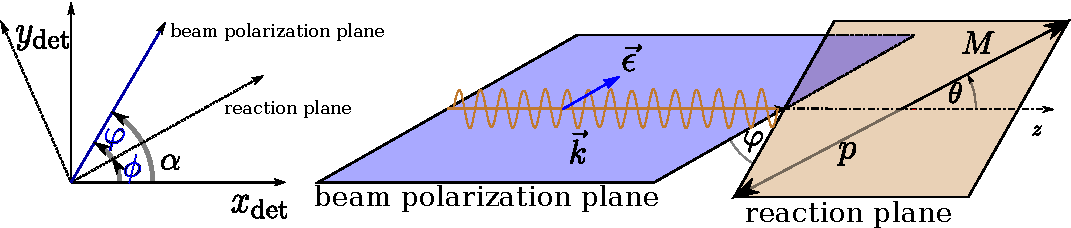
\includegraphics[width=\linewidth]{../DPG2022/figs/angles.pdf}
	\caption{Left: Definition of angles $\alpha,\phi,\varphi$. Right: Photon momentum $\vec{k}$ and polarization  $\vec{\epsilon}$ define the beam polarization plane while the reaction plane is defined by the recoil proton $p$ and produced meson $M$.}
	\label{fig:angles}
\end{figure} 
Theoretically the beam asymmetry can be determined by a measurement of the cross section and a fit using equation \eqref{eq:asym}. However, when calculating polarized cross sections, it is important to have good control over flux normalization and detector acceptance in three dimensions $(E_\gamma,\cos\theta,\phi)$. To avoid this, the measurement of asymmetries can be used to access the polarization observable $\Sigma$ instead. Particularly, data is taken for two distinct orthogonal polarization settings corresponding to $\alpha=\pm\SI{45}{\degree}$.

This chapter will illustrate the process of determining the beam asymmetry for $\eta$ and $\eta'$ photoproduction. The published results of $\Sigma_{\eta}$ \cite{farahphd,eta} are used to check the accuracy and functionality of employed bayesian methods. Bayesian methods, as well as traditional frequentist approaches are used afterwards to extract new results for $\Sigma_{\eta'}$. First, the used methods will be presented and subsequently their application for each final state, respectively.
\section{Methods}
\label{sec:meth}
The beam asymmetry has to be determined via fits to $\phi$ distributions obtained from data. These are performed as either binned or unbinned fits. Both methods allow the application of Bayesian methods as will be discussed in the following. Additionally the advantages and disadvantages off all methods are compared.
\subsection{Event yield asymmetries}
Measurements were made in two distinct polarization settings $\alpha=\pm\SI{45}{\degree}=\alpha^{\bot/\parallel}$. Thus, the polarized cross sections for both settings are given by\footnote{The dependencies of polarized and unpolarized cross sections as well as the beam asymmetry like in equation \eqref{eq:asym} are implied}
\begin{equation}
	\frac{\text{d}\sigma}{\text{d}\Omega}_\text{pol}^\parallel=\frac{\text{d}\sigma}{\text{d}\Omega}_0\cdot\left[1-p_\gamma^\parallel\Sigma\cos\left(2\left(\alpha^\parallel-\phi\right)\right)\right]
	\label{eq:polcs0}
\end{equation}
and 
\begin{align}
	\frac{\text{d}\sigma}{\text{d}\Omega}_\text{pol}^\bot&=\frac{\text{d}\sigma}{\text{d}\Omega}_0\cdot\left[1-p_\gamma^\bot\Sigma\cos\left(2\left(\alpha^\bot-\phi\right)\right)\right]\label{eq:polcs00}\\
	&=\frac{\text{d}\sigma}{\text{d}\Omega}_0\cdot\left[1+p_\gamma^\bot\Sigma\cos\left(2\left(\alpha^\parallel-\phi\right)\right)\right].\label{eq:polcs}
\end{align}
Note that equation \eqref{eq:polcs} holds, because 
\begin{align*}
	\alpha^\bot=\alpha^\parallel+\pi/2 &&\text{and}&&\cos x = -1\cdot\cos(x+\pi).
\end{align*}
Consider now taking the difference of equations \eqref{eq:polcs0} and \eqref{eq:polcs}
\begin{equation}
	\frac{\text{d}\sigma}{\text{d}\Omega}_\text{pol}^\bot-\frac{\text{d}\sigma}{\text{d}\Omega}_\text{pol}^\parallel=\frac{\text{d}\sigma}{\text{d}\Omega}_0\cdot\left(p_\gamma^\bot+p_\gamma^\parallel\right)\Sigma\cos\left(2\left(\alpha^\parallel-\phi\right)\right).
\end{equation}
One can further eliminate the unpolarized cross section from this equation by dividing by the polarization weighted sum of equations \eqref{eq:polcs0} and \eqref{eq:polcs}
\begin{equation}
	\alpha\cdot\frac{\text{d}\sigma}{\text{d}\Omega}_\text{pol}^\parallel+\beta\cdot\frac{\text{d}\sigma}{\text{d}\Omega}_\text{pol}^\bot=\frac{\text{d}\sigma}{\text{d}\Omega}_0\cdot\left[\alpha+\beta-\left(\alpha p_\gamma^\parallel-\beta p_\gamma^\bot\right)\Sigma\cos\left(2\left(\alpha^\bot-\phi\right)\right)\right]\overset{!}{=}2\frac{\text{d}\sigma}{\text{d}\Omega}_0.
\end{equation}
Since $$\frac{\text{d}}{\text{d}\phi}\frac{\text{d}\sigma}{\text{d}\Omega}_0\overset{!}{=}0\forall\phi,$$ it holds \begin{align}
	\alpha p_\gamma^\parallel-\beta p_\gamma^\bot \overset{!}{=}0 && \alpha+\beta\overset{!}{=}2,
\end{align}
such that
\begin{align}
	\alpha =\frac{2p_\gamma^\parallel}{p_\gamma^\bot+p_\gamma^\parallel} && \beta=\frac{2p_\gamma^\bot}{p_\gamma^\bot+p_\gamma^\parallel}.
	\label{eq:alphabeta}
\end{align}
The beam asymmetry $\Sigma$ is thus accessible via the asymmetry \begin{equation}
	A(\phi)=\frac{\frac{\text{d}\sigma}{\text{d}\Omega}_\text{pol}^\bot-\frac{\text{d}\sigma}{\text{d}\Omega}_\text{pol}^\parallel}{p_\gamma^\parallel\frac{\text{d}\sigma}{\text{d}\Omega}_\text{pol}^\bot+p_\gamma^\bot\frac{\text{d}\sigma}{\text{d}\Omega}_\text{pol}^\parallel}=\Sigma\cos\left(2\left(\alpha^\parallel-\phi\right)\right).
	\label{eq:asymfit}
\end{equation}
At this point one can now make use of the fact that in any scattering reaction the number of events $N$ is given by the product of luminosity $L$ and total cross section $\sigma$ $$N=L\cdot\sigma=\Phi\cdot N_t\cdot\frac{\text{d}\sigma}{\text{d}\Omega}\cdot\Delta\Omega,$$
where $\Phi$ is the beam flux, $N_t$ the number of target particles and $\Delta\Omega$ is the solid angle covered by the detector. Substituting this in equation \eqref{eq:asymfit} one can build the asymmetry $A(\phi)$ using only the (flux-)normalized event yields $\tilde{N}^{\parallel/\bot}\left(E_\gamma,\cos\theta,\phi\right)$\footnote{again, arguments $\left(E_\gamma,\cos\theta,\phi\right)$ are implied.}
\begin{equation}
	A(\phi)=\frac{\tilde{N}^\bot-\tilde{N}^\parallel}{p_\gamma^\parallel\tilde{N}^\bot+p_\gamma^\bot\tilde{N}^\parallel}=\Sigma\cos\left(2\left(\alpha^\parallel-\phi\right)\right).
	\label{eq:evyieldasym}
\end{equation}
Alternatively, the event yields $N$ can also be normalized by integrating over the total azimuthal angle range in each bin of $(E_\gamma,\cos\theta)$. This normalization technique has been used in reference \cite{farahphd} and will also be used in this work. Using appropriate binning in $\phi$ in addition to beam energy and meson polar angle the asymmetry can be build for all kinematic bins and the beam asymmetry then be extracted via a one-Parameter fit. The statistical errors for $A(\phi)$ are given by \textsc{Gaussian} error propagation (see appendix \ref{sec:stat_err}). 
\subsubsection{Frequentist}
The beam asymmetry can now be determined via a frequentist fit, where $\Sigma$ is determined such that the $\chi^2$ value resulting from the data points and equation \ref{eq:evyieldasym} is minimized. The results are point estimates with statistical error bars that are also obtained from the fit: $\hat{\Sigma}\pm\sigma_{\hat{\Sigma}}$. In addition $\chi^2/\text{NDF}\approx1$ may be verified in order to diagnose the fit itself. Multiple automated minimization and calculation algorithms for $\chi^2$ fitting are available as open source. The \emph{Python} \cite{python} module \emph{scipy} \cite{scipy} and \emph{ROOT} \cite{root} offer e.g. the methods \texttt{scipy.optimize.curve\_fit} \cite{pFit} and \texttt{TH1::Fit()} \cite{rFit} for discrete/binned data, which were used in the analysis.
\subsubsection{\textsc{Bayesian}}
Following section \ref{sec:bayes}, where the basics of \textsc{Bayesian} inference were discussed, the goal of a \textsc{Bayesian} approach is to sample marginal posterior distributions for each fitted parameter from the joint posterior $p(\boldsymbol{\theta}|y)$ which depends on the observed data $y$. The joint posterior itself is proportional to the product of priors $\pi(\boldsymbol{\theta})$ and likelihood $\mathcal{L}(y|\boldsymbol{\theta})$ (\textsc{Bayes'} theorem). This collapses to a one parameter problem in the case of fitting the event yield asymmetries (Eq. \eqref{eq:evyieldasym})
\begin{equation}
	p(\Sigma|y)\propto \pi({\Sigma})\cdot \mathcal{L}(y|\Sigma).
\end{equation}
However, to be able to sample from a joint posterior, prior and likelihood need to be specified. In order not to bias the fit towards any particular values, the prior is chosen non-informative, realized by a broad \textsc{Gaussian} centered at 0 which is truncated to the physically allowed parameter space of $\Sigma\in[-1,1]$. Furthermore, the likelihood is formulated assuming \textsc{Gaussian} errors $\epsilon_n$ at each data point $y_n$, which should be described by the asymmetry (Eq \eqref{eq:evyieldasym}) at bin $n$ $A(\phi_n;\Sigma)$, i. e. \footnote{Remember the notation introduced in section \ref{sec:bayes}: $x\sim\mathcal{N}(\mu,\sigma)=\mathcal{N}(x|\mu,\sigma)=\frac{1}{\sqrt{2\pi\sigma^2}}e^{-\frac{(x-\mu)^2}{2\sigma^2}}$}
\begin{align}
	\Sigma \sim \mathcal{N}\left(0,1\right)_{[-1,1]} && y_n=A\left(\phi_n;\Sigma\right)+\epsilon_n && \epsilon_n\sim\mathcal{N}\left(0,\sigma_n\right),
\end{align}
which is equivalent to
\begin{align}
	 \Sigma \sim \mathcal{N}(0,1) &&y_n\sim\mathcal{N}\left(A(\phi_n;\Sigma),\sigma_n\right).
\end{align}
The likelihood of all data points now evaluates to the product of the likelihood at each data point $y_n$ and the posterior results in \begin{align}
	p(\Sigma|y)&\propto\pi(\Sigma)\cdot\mathcal{L}(y|\Sigma)=\mathcal{N}\left(\Sigma|0,1\right)_{[-1,1]}\cdot\prod_{n}\mathcal{N}\left(y_n|A\left(\phi_n;\Sigma\right),\sigma_n\right)\\
	\Leftrightarrow -\ln p(\Sigma|y)&=\frac{1}{2}\Sigma^2+\frac{1}{2}\sum_{n}\left(\frac{y_n-A\left(\phi_n;\Sigma\right)}{\sigma_n}\right)^2+\text{ constant terms }, 
\end{align}
such that all ingredients are present to form a fully \textsc{Bayesian} probabilistic model\footnote{Note that the sampling aims only to reflect the right proportionality of the (marginal) posterior. Thus, constant terms can be dropped and are of no further interest \cite{stan}.}. This model was implemented in Stan \cite{stan}, directly giving access to samples from the posterior obtained with the No-U-Turn-Sampler (NUTS) \cite{stan,nuts}. Hereby, the sampling is restricted to the allowed parameter region $\Sigma\in[-1,1]$. As a measure of goodness of fit, the $p$-values obtained from the posterior predictive distributions, as introduced in section \ref{sec:bayes}, are reviewed. To diagnose the convergence of the MCMC fit, sensible values for $\hat{R}$ and the Monte-Carlo standard error $\sigma_\text{MCSE}$ are verified.
\subsection{Event based fit}
Although intuitive and easily implementable the binned fit --\textsc{Bayesian} or not-- has one critical disadvantage: it is inevitable that information is lost because the asymmetry $A(\phi)$ is a binned quantity and hence, the choice of binning influences the fit results. This is discussed in more detail in appendix \ref{app:binnedfits}. Especially kinematic bins with low statistics show this behavior. To circumvent this problem, an \emph{unbinned fit}, based on the likelihood function for each event, can be performed. Also, no assumptions on the distribution of statistical errors have to be made since each event is taken into account individually. Yet, the event based fit does not provide any measure of goodness of fit, so that the study of toy Monte Carlo data is essential when checking the working principle of the method.

In a polarized experiment the azimuthal angle distribution of events is not isotropic, but modulated by a cosine term coupling to beam asymmetry $\Sigma$ and beam polarization $p_\gamma^{\parallel/\bot}$ for each setting $\alpha^{\parallel/\bot}$, as is expressed through the respective differential cross sections in Equations \ref{eq:polcs0} and \ref{eq:polcs00}. Since the number of events is proportional to the cross section, the probability $p\left(\phi,p_\gamma^{\parallel/\bot}|\Sigma\right)$ to find an event under the azimuthal angle $\phi$ for a given bin of $\left(E_\gamma,\cos\theta\right)$ and setting $\alpha^{\parallel/\bot}$ is \footnote{Note: Normalizing $p\left(\phi,p_\gamma^{\parallel/\bot}\big|\Sigma\right)$ to $2\pi$ (or any other arbitrary constant) is sufficient for the fit as long as the integral does not depend on the fit parameters. The normalization to $2\pi$ is chosen for better readability. However, to calculate actual probabilities, one must multiply Eq. \eqref{eq:prob0} by $2\pi$.} \begin{equation}
	p\left(\phi,p_\gamma^{\parallel/\bot}\big|\Sigma\right)=\frac{\left[1\mp p_\gamma^{\parallel/\bot}\Sigma\cos\left(2\left(\alpha^\parallel-\phi\right)\right)\right]}{\frac{1}{2\pi}\int_{0}^{2\pi}\text{d}\phi\left[1\mp p_\gamma^{\parallel/\bot}\Sigma\cos\left(2\left(\alpha^\parallel-\phi\right)\right)\right] }.
	\label{eq:prob0}
\end{equation}
This is only true for an idealized experiment with acceptance $\epsilon=\text{const}\forall\phi$, so that the acceptance $\epsilon(\phi)$ has to be included in the probability for each event. As demonstrated in reference \cite{hartmannphd} a \textsc{Fourier} series truncated after the fourth order is sufficient to model any occurring function $$\epsilon\left(\phi\right)=\sum_{k=0}^4a_k\sin\left( k\phi\right)+b_k\cos\left(k\phi\right),$$ where the eight detector coefficients $a_k$ and $b_k$ are determined from the fit. With this the measurable probability $\tilde{p}\left(\phi,p_\gamma^{\parallel/\bot}\big|\Sigma,a,b\right)$ is 
\begin{align}
	\tilde{p}\left(\phi,p_\gamma^{\parallel/\bot}\big|\Sigma,a,b\right)&\propto\left[1\mp p_\gamma^{\parallel/\bot}\Sigma\cos\left(2\left(\alpha^\parallel-\phi\right)\right)\right]\cdot\epsilon(\phi)\\&=\left[1\mp p_\gamma^{\parallel/\bot}\Sigma\cos\left(2\left(\alpha^\parallel-\phi\right)\right)\right]\cdot\left(\sum_{k=0}^4a_k\sin\left( k\phi\right)+b_k\cos\left(k\phi\right)\right),
\end{align}
where $a:=\{a_k\}_{k=0}^4, b:=\{b_k\}_{k=0}^4$.Finally, normalizing $\frac{1}{2\pi}\int_{0}^{2\pi}\text{d}\phi\tilde{p}\left(\phi,p_\gamma^{\parallel/\bot}\big|\Sigma,a,b\right)\overset{!}{=}1$,
\begin{equation}
	\tilde{p}\left(\phi,p_\gamma^{\parallel/\bot}\big|\Sigma,a,b\right)=\frac{\left[1\mp p_\gamma^{\parallel/\bot}\Sigma\cos\left(2\left(\alpha^\parallel-\phi\right)\right)\right]\cdot\left(\sum_{k=0}^4a_k\sin\left( k\phi\right)+b_k\cos\left(k\phi\right)\right)}{1\pm\frac{1}{2}a_2p_\gamma^{\parallel/\bot}\Sigma}.
	\label{eq:prob}
\end{equation}
The respective polarization setting $\alpha^{\parallel/\bot}$ determines the sign in the normalizing constant which allows an uncorrelated estimation of the detector coefficient $a_2$ and the beam asymmetry $\Sigma$. To simplify notation and implementation, Equation \eqref{eq:prob} can be written as \emph{one} probability for all events -- irregardless of polarization setting -- if the polarization values $p_\gamma^\parallel$ are multiplied by $(-1)$ and summarized as $p_\gamma$: \begin{equation}
	\tilde{p}\left(\phi,p_\gamma\big|\Sigma,a,b\right)=\frac{\left[1+p_\gamma\Sigma\cos\left(2\left(\alpha-\phi\right)\right)\right]\cdot\left(\sum_{k=0}^4a_k\sin\left( k\phi\right)+b_k\cos\left(k\phi\right)\right)}{1-\frac{1}{2}a_2p_\gamma\Sigma},
	\label{eq:prob}
\end{equation} 
with $\alpha=\SI{-45}{\degree}$ fixed.

In section \ref{sec:time} the subtraction of uncorrelated time background was discussed via a sideband subtraction. Naturally, without binning the data, this strategy is invalid and prompt peak and sideband events have to be fitted simultaneously. Hereby it is important to consider that the random time background is realized as flat distribution underneath the complete reaction time spectrum (cf. Figure \ref{fig:time_r}), \emph{including} the range of the prompt peak. The fraction of true coincident events to random coincidences is given as \begin{equation}
	f=\frac{N_\text{prompt}-w\cdot N_\text{sideband}}{N_\text{prompt}},
\end{equation}
where $N_\text{prompt}$ and $N_\text{sideband}$ are the number of events where the reaction time lies within the prompt peak or sideband, respectively. $w$ is the ratio of the widths of the chosen prompt peak and sideband
ranges, see section \ref{sec:time}. It is now assumed that the random coincidences will exhibit an asymmetry $\Sigma^\text{bkg}$ of their own and are not necessarily described by the detector coefficients $a$ and $b$ but rather by $a^\text{bkg}$ and $b^\text{bkg}$. The probability to detect a prompt peak event $p_\text{prompt}$ and the probability to measure a sideband event $p_\text{sideband}$ are then given by 
\begin{align}
p_\text{prompt}\left(\phi,p_\gamma,\big|\Sigma,a,b,\Sigma^\text{bkg},a^\text{bkg},b^\text{bkg}\right)&=f\cdot\tilde{p}\left(\phi,p_\gamma\big|\Sigma,a,b\right)+\left(1-f\right)\cdot\tilde{p}\left(\phi,p_\gamma\big|\Sigma^\text{bkg},a^\text{bkg},b^\text{bkg}\right)\label{eq:pprmpt}\\
p_\text{sideband}\left(\phi,p_\gamma\big|\Sigma^\text{bkg},a^\text{bkg},b^\text{bkg}\right)&=\tilde{p}\left(\phi,p_\gamma\big|\Sigma^\text{bkg},a^\text{bkg},b^\text{bkg}\right)\label{eq:pside}.
\end{align}
If there are $n$ prompt peak and $m$ sideband events, the joint likelihood of all events $\mathcal{L}$ is thus given by
\begin{equation}
	\mathcal{L}=\prod_{i=1}^{n}p_\text{prompt}\left(\phi_i,p_{\gamma,i}\big|\Sigma,a,b,\Sigma^\text{bkg},a^\text{bkg},b^\text{bkg}\right)\prod_{j=1}^mp_\text{sideband}\left(\phi_j,p_{\gamma,j}\big|\Sigma,a,b,\Sigma^\text{bkg},a^\text{bkg},b^\text{bkg}\right),
\end{equation}
or, equivalently
\begin{equation}
\begin{aligned}
	\ln\mathcal{L}&=\sum_{i=1}^{n}\ln p_\text{prompt}\left(\phi_i,p_{\gamma,i}\big|\Sigma,a,b,\Sigma^\text{bkg},a^\text{bkg},b^\text{bkg}\right)\\&+\sum_{j=1}^m \ln p_\text{sideband}\left(\phi_j,p_{\gamma,j}\big|\Sigma,a,b,\Sigma^\text{bkg},a^\text{bkg},b^\text{bkg}\right).\label{eq:lik}
\end{aligned}
\end{equation}
Eighteen\footnote{The \textsc{Fourier} series is constructed such that $a_0=0,b_0=1$} parameters have to be determined in total, either via a conventional frequentist approach or a \textsc{Bayesian} approach to this non-linear fitting problem.
\subsubsection{Frequentist}
Best fit estimates can be derived by maximizing the likelihood $\mathcal{L}$, or, for computational convenience, by minimizing $-\ln\mathcal{L}$. The \emph{ROOT} library \cite{root} offers the method \emph{TTree::UnbinnedFit} to perform an unbinned maximum likelihood fit on data filled in a \emph{TTree} \cite{runbinnedFit}, which was used to perform the fit. Minimization and statistical error calculation are performed by \emph{MINUIT} \cite{minuit}. Errors are hereby estimated either symmetrical from the paraboloid shape of $(-\ln\mathcal{L})$ using the \emph{HESSE} algorithm or asymmetric from the half-maximum values of $(-\ln\mathcal{L})$ using the \emph{MINOS} algorithm without making assumptions on the shape of the likelihood, if necessary \cite{minuit}.  
\subsubsection{Bayesian}
The joint posterior of all fit parameters given the data $\phi,p_\gamma$ is 
\begin{equation}
	p\left(\Sigma,a,b,\Sigma^\text{bkg},a^\text{bkg},b^\text{bkg}\big|\phi,p_\gamma\right)\propto \mathcal{L}\left(\phi,p_\gamma\big|\Sigma,a,b,\Sigma^\text{bkg},a^\text{bkg},b^\text{bkg}\right)\cdot\pi\left(\Sigma,a,b,\Sigma^\text{bkg},a^\text{bkg},b^\text{bkg}\right),
\end{equation}
where $\pi(\boldsymbol{\theta})$ denotes the combined prior of all fit parameters which factors into each individual prior since all parameters are independent:
\begin{equation}
	\pi\left(\Sigma,a,b,\Sigma^\text{bkg},a^\text{bkg},b^\text{bkg}\right)=\pi\left(\Sigma\right)\cdot\pi\left(a\right)\cdot\pi\left(b\right)\cdot\pi\left(\Sigma^\text{bkg}\right)\cdot\pi\left(a^\text{bkg}\right)\cdot\pi\left(b^\text{bkg}\right).
\end{equation}
The priors for $\Xi\in\{\Sigma,\Sigma^\text{bkg}\}$ and $\xi\in\{a,b,a^\text{bkg},b^\text{bkg}\}$ are again chosen non-informative, broadly centered around 0
\begin{align}
	\Xi\sim\mathcal{N}(0,1)_{[-1,1]} &&\xi_k\sim\mathcal{N}(0,0.1).
	\label{eq:priors}
\end{align}
This model, consisting of the likelihood in Eq. \eqref{eq:lik} and the priors in Eq. \eqref{eq:priors}, is implemented in Stan \cite{stan}, so that samples from the posterior in the physically allowed region ($\Xi\in[-1,1]$) are again obtained via NUTS \cite{nuts}. From references \cite{farahphd,hartmannphd} it  is expected that $\xi_k\ll1$, therefore the chosen widths of the priors resemble a, relatively speaking, broad distribution.
\subsection{Comparison of \textsc{Bayesian} and frequentist approaches}
\label{sec:sigma_eta}
The effort of implementing the binned or unbinned fit in a \textsc{Bayesian} approach is comparable to the traditionally used frequentist methods. Due to the probabilistic structure of the Stan language \cite{stan} implementation of likelihood and prior models is straightforward and the sampling algorithms can be accessed or modified to ones needs intuitively. However, the \textsc{Bayesian} fit requires more careful preparation and also diagnostics. On one hand, the choice of priors has to be made. On the other hand, the fitting procedure is inherently different; not only the goodness of fit (compared with data) has to be checked but also the convergence of the \textsc{Markov} chains themselves. Yet, the additional effort is rewarded by the fact that the \textsc{Bayesian} fit will yield \emph{distributions} for all parameters as opposed to point estimates with error bars. This is especially useful for polarization observables which may be used as input for PWA calculations. Here error estimates can be derived from the distributions e.g. as (multiple) standard deviations, the full width at half maximum or similar. If furthermore a \textsc{Bayesian} approach is  pursued, also the whole distributions may be used. Another advantage of the \textsc{Bayesian} fit is the ability to truncate the posterior samples to the relevant or allowed parameter space.      

\section{Determination of $\Sigma_{\eta}$ using Bayesian statistics}
This section will now demonstrate the application of the discussed methods to obtain the beam asymmetry $\Sigma$ for $\eta$ photoproduction with selected data provided from reference \cite{farahphd}. For each method only the respective \textsc{Bayesian} approach will be used and compared to the results from \cite{farahphd} to confirm the that it is a valid method. As an additional sanity check toy Monte Carlo samples are generated and analyzed. 
\subsection{Application of methods to toy Monte Carlo data}
Although results can be compared to the already accomplished ones in reference \cite{farahphd}, verifying the correct functioning of the fitting methods is still useful. This is done by generating events that follow the expected distributions of $N^{\parallel/\bot}$ with fixed and known parameters. With the simulated event yields the binned and unbinned fit are performed as described previously. Repeating this for a large number of times should reproduce the input parameters if the methods work as intended.
\subsubsection{Event yield asymmetries}
The asymmetry $A\left(\phi\right)$ is built from the event yields $N^{\parallel/\bot}$, which are distributed according to
\begin{align}
	N^{\parallel}=N_0\left[1-p_\gamma^\parallel\Sigma\cos\left(2\left(\alpha^\parallel-\phi\right)\right)\right],\label{eq:npar}\\
	N^{\bot}=N_0\left[1-p_\gamma^\bot\Sigma\cos\left(2\left(\alpha^\bot-\phi\right)\right)\right],
	\label{eq:nbot}
\end{align}
where the parameters are chosen as $\Sigma=0.3,p_\gamma^\parallel=0.25,p_\gamma^\bot=0.3$. In each toy Monte Carlo bin the number of generated samples per setting $N_\text{total}^{\parallel/\bot}$ is given by a \textsc{Poisson} distribution
\begin{align}
N_\text{total}^\parallel \sim \mathcal{P}(800) && N_\text{total}^\bot \sim \mathcal{P}(1000),
\end{align}
to simulate the statistics of the $\gamma p \to p\eta$ final state as accurately as possible \cite{farahphd}. The samples from the distributions \eqref{eq:npar},\eqref{eq:nbot} are drawn using the \emph{TH1::GetRandom} \cite{rrandom} function provided by \emph{ROOT} \cite{root}. The function from which samples should be drawn is integrated point wise and then normalized. The normalized integral is approximated by a parabola for each bin. A random number between 0 and 1 is generated and assigned to the according bin, where the respective parabola is evaluated to give the desired random value. \cite{rrandom}.

\begin{landscape}
	\begin{figure}[htbp]
		\centering
		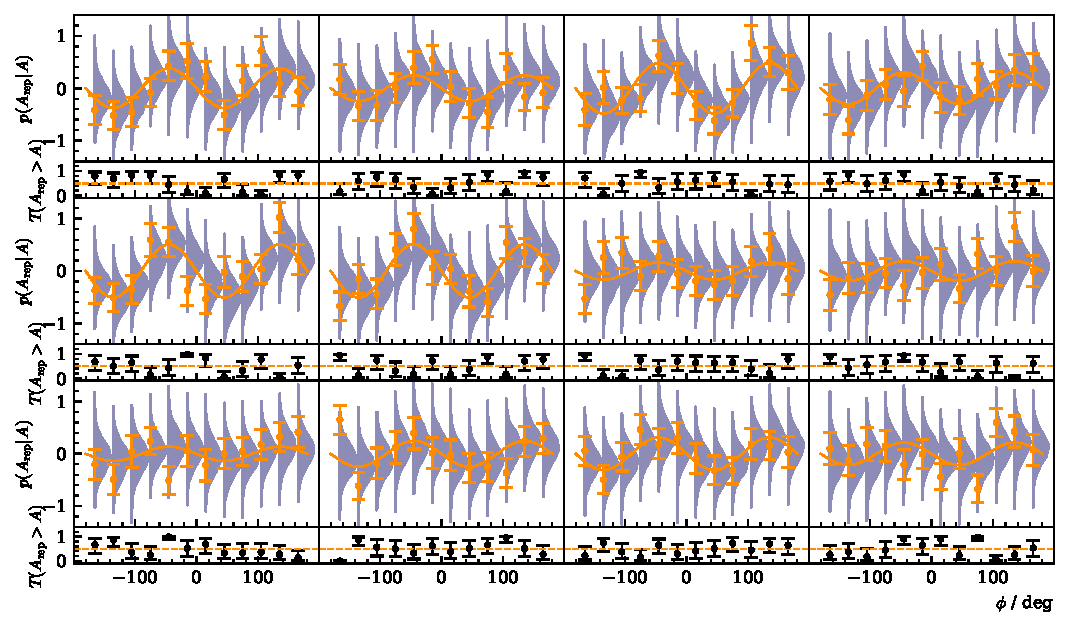
\includegraphics[width=\linewidth,height=.8\textwidth]{../bayes/toyMC/plots/toyMC_ppd_checks.pdf}
		\caption{Posterior predictive checks $p\left(A_\text{rep}\big|A\right)$ from a \textsc{Bayesian} fit to the event yield asymmetries for six toy Monte Carlo bins are shown as distributions. The black data points are the asymmetry $A\left(\phi\right)$, which was additionally fitted using a $\chi^2$ fit (solid red line). The goodness of fit is shown using $p$-values, which give the fraction $T\left(A_\text{rep}>A\right)$ of replicated samples greater than the original measured value, with propagated statistical error bars on the bottom of each plot. The expected mean value of $T\left(A_\text{rep}>A\right)=0.5$ is indicated by the dashed red line. }
		\label{fig:toymc_asym}
	\end{figure}
\end{landscape}

\noindent In total, 10000 toy Monte Carlo bins were simulated and the asymmetry built for $12$ bins in $\phi$, to conform with the binning chosen in reference \cite{farahphd}. The resulting asymmetry $A\left(\phi\right)$ is shown in Figure \ref{fig:toymc_asym} for several bins as the orange data points with statistical errors according to \textsc{Gaussian} error propagation. Additionally shown is a $\chi^2$ fit (red line) to the asymmetry together with posterior predictive checks as obtained from a fully \textsc{Bayesian} fit according to the introduced model (distributions). This \textsc{Bayesian} fit was performed employing $n_\text{chain}=4$ \textsc{Markov} chains with $n_\text{samples}=1000$ samples each. The warm-up period for each chain has the same length of $n_\text{warm up}=1000$
\begin{align}
	n_\text{chain}=4 && n_\text{samples}=1000 && n_\text{warm up}=1000.
\end{align}
The goodness of fit is checked via the introduced $p$-values $p=T(A_\text{rep}>A)$, and are shown as black points with propagated error bars on the bottom. The optimal value of $p=0.5$ is marked by the red, dashed line and realizes the mean of the distribution of all $p$-values, so that one can assume good description of the data by the fits, see Figure \ref{fig:toymc_pvals}. This replaces the investigation of the $\chi^2/\text{NDF}$ distribution in the case of a frequentist fit, which should have a mean of $1$.  
\begin{figure}[htbp]
	\centering
	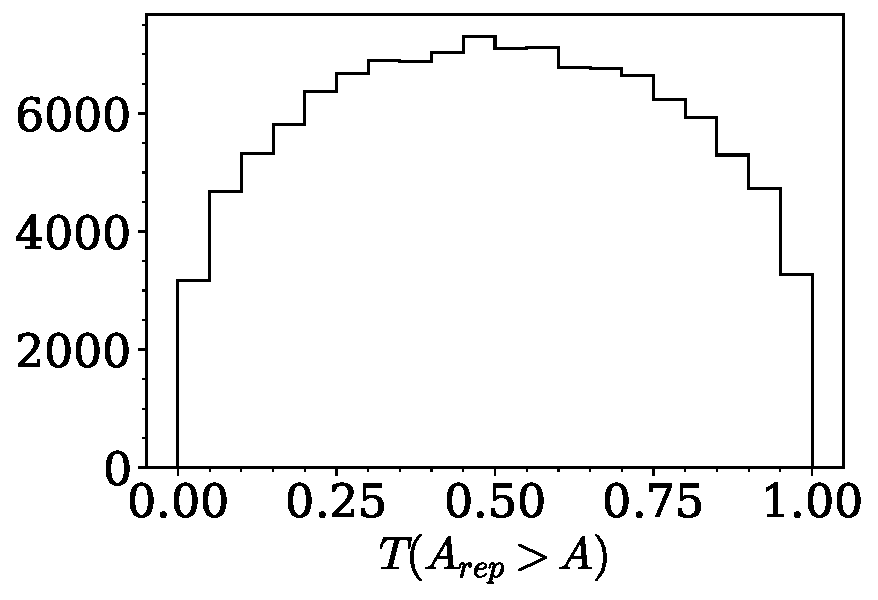
\includegraphics[width=\linewidth]{../bayes/toyMC/plots/toyMC_pval_hist.pdf}
	\caption{$p$ values of all toy Monte Carlo bins. They are centered around their mean at $0.5$, which is indicated by the dashed line, and show no bias towards higher or lower values, thus confirming an adequate fit.}
	\label{fig:toymc_pvals}
\end{figure}

\noindent To check whether the fit is unbiased and provides correct error estimation one can investigate the normalized residuals
\begin{equation}
	\xi = \frac{\Sigma^\text{fit}-\Sigma^\text{true}}{\Delta\Sigma^\text{fit}}
	\label{eq:res}
\end{equation}
 in the case of a least-squares fit. Here $\Sigma^\text{fit}$ and $\Delta\Sigma^\text{fit}$ are the value and corresponding statistical error for the beam asymmetry as obtained from the fit and $\Sigma^\text{true}$ is the true value that was used to throw the toy MC experiments. An unbiased fit with right estimation of errors yields \cite{statistics} \begin{equation}
	\xi\sim\mathcal{N}\left(0,1\right).
	\label{eq:xi}
\end{equation}
This criterion obviously cannot be applied in the same way to a \textsc{Bayesian} fit. The fit results are distributions and therefore lack point estimates $\Sigma^\text{fit}$ and errors $\Delta\Sigma^\text{fit}$. However, one can modify Equation \eqref{eq:res} to the needs of a \textsc{Bayesian} fit to assess its performance:
\begin{equation}
	\Xi=\frac{\left\{\Sigma^\text{fit}\right\}-\Sigma^\text{true}}{\text{std}\left(\left\{\Sigma^\text{fit}\right\}\right)}\sim\mathcal{N}(0,\sigma).
\end{equation}
Instead of the point estimates $\Sigma^\text{fit}$ the set of all draws from the marginal posteriors $\left\{\Sigma^\text{fit}\right\}$ is shifted by the true value $\Sigma_\text{true}$ and normalized by the standard deviation as an error estimate for each fit. Although this is not a rigorously derived quantity it allows to identify possible bias if $\text{mean}\left(\Xi\right)\neq 0$. Furthermore, checking that $\sigma\approx1$ will affirm whether the width of the marginal posterior distributions is sensible. Figure \ref{fig:toymcpost} shows the combined $\Xi$-distributions of all fits and the unaltered combined posteriors shifted by the true value. As expected, both distributions are normal as a \textsc{Gaussian} fit proves.  
\begin{figure}[htbp]
	\centering
	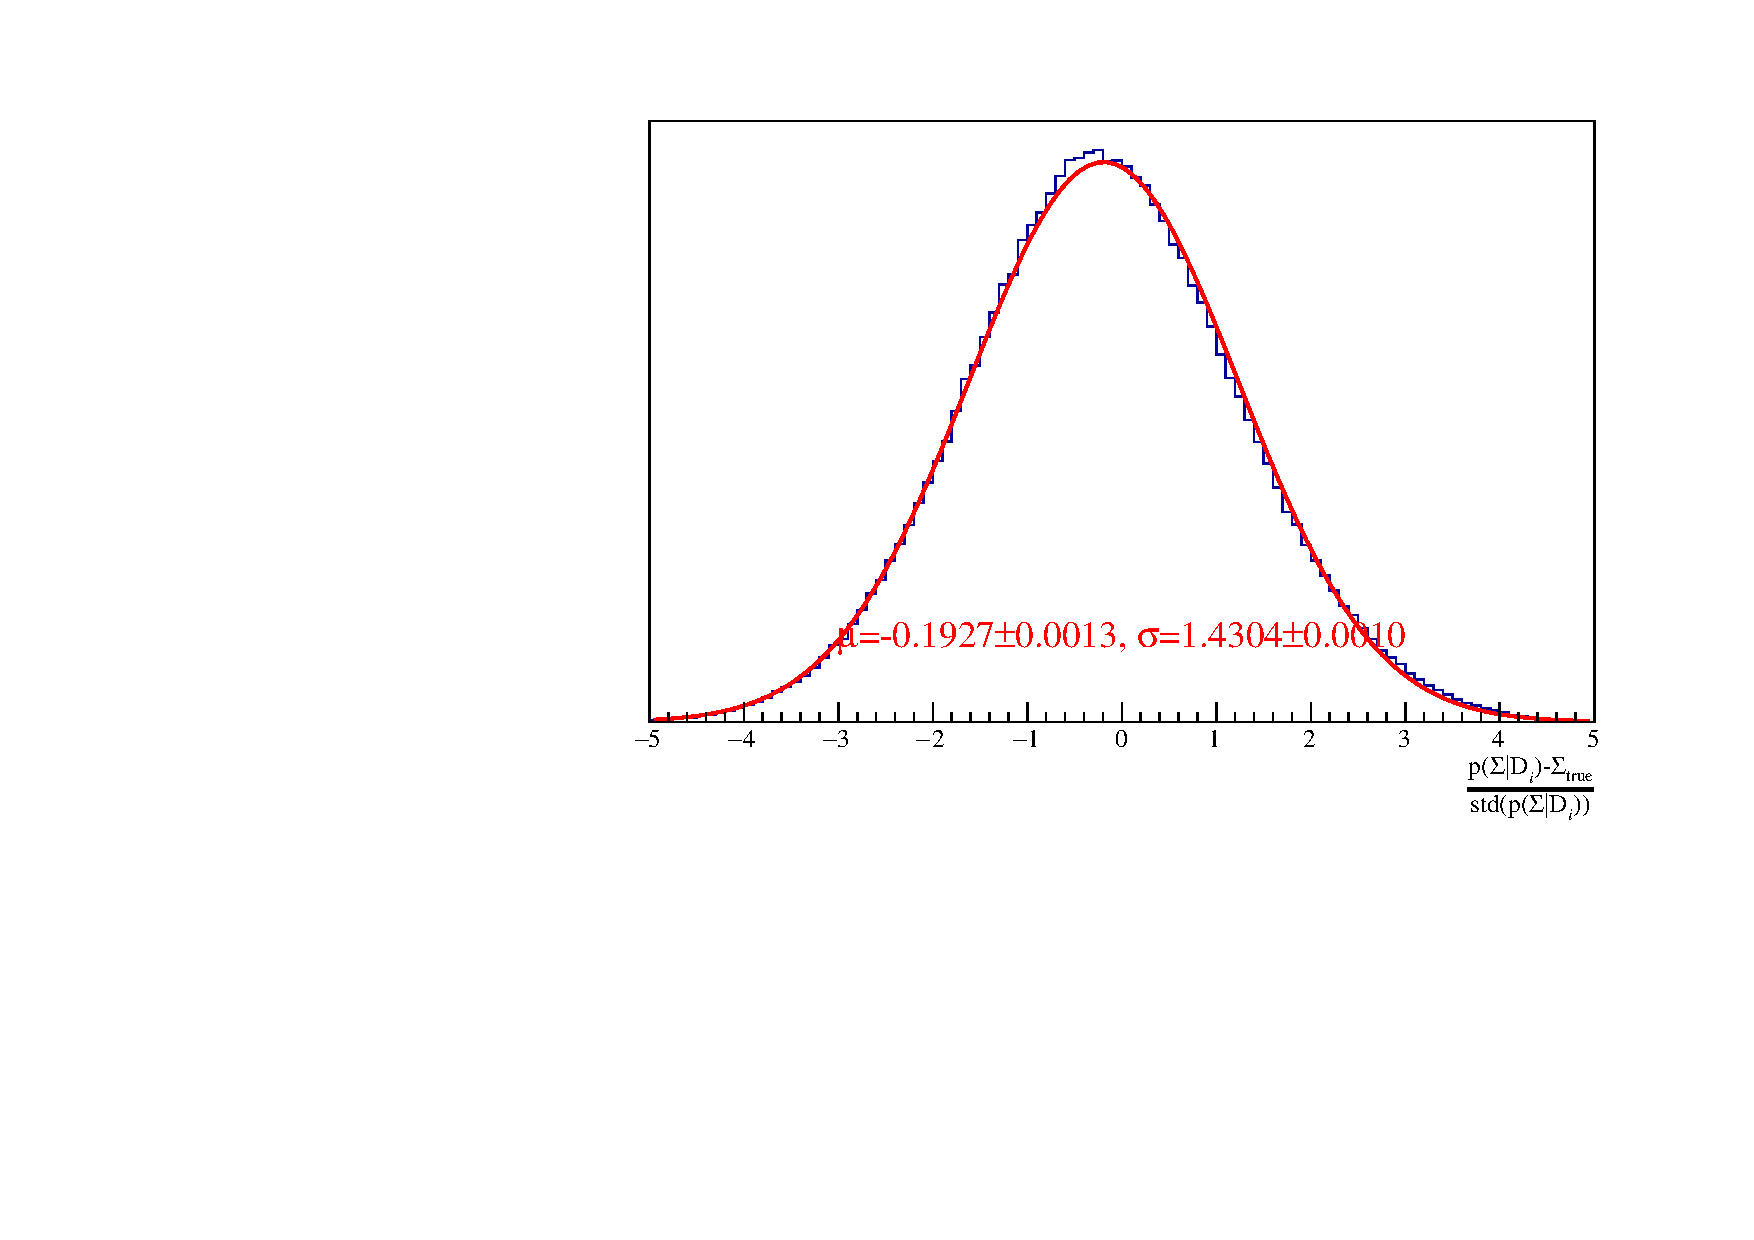
\includegraphics[width=.49\linewidth]{../bayes/toyMC/plots/combined_post_add.pdf}
	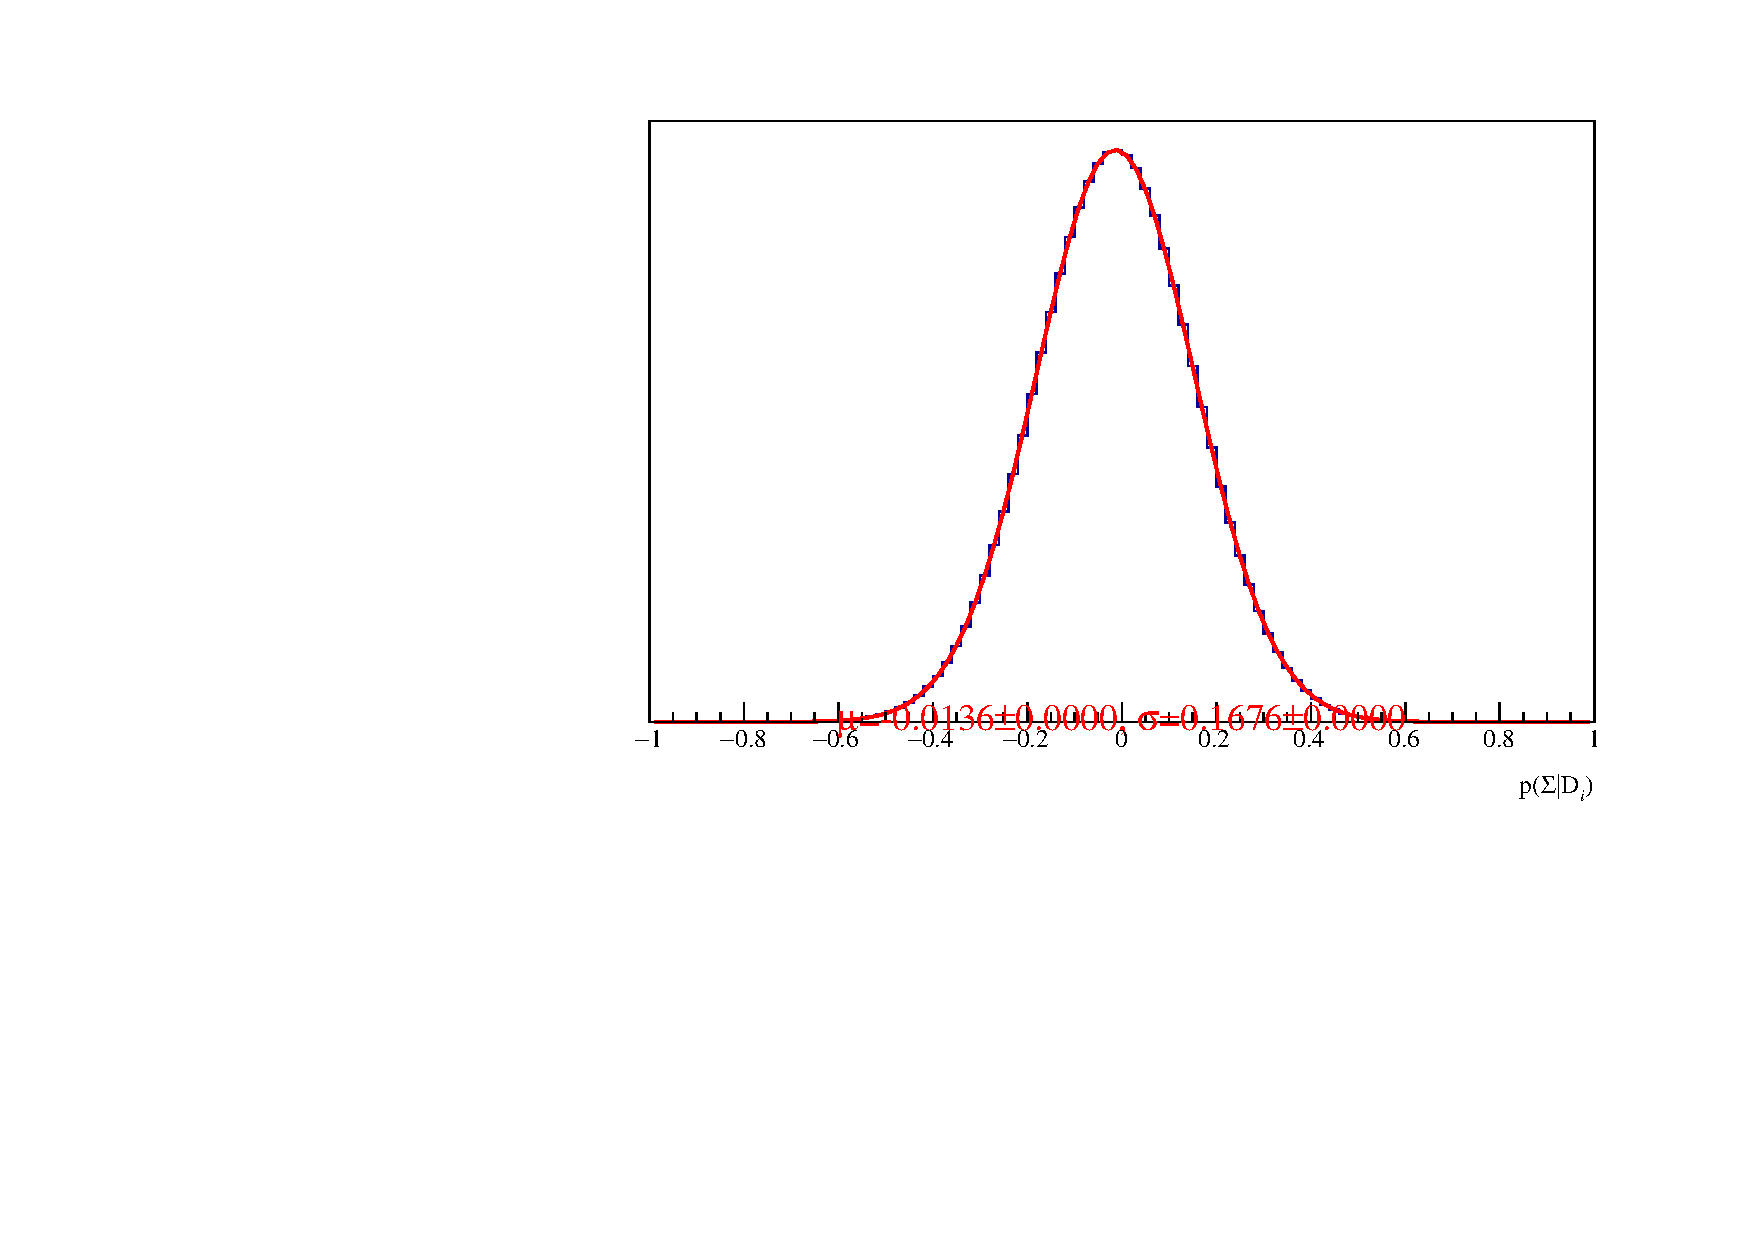
\includegraphics[width=.49\linewidth]{../bayes/toyMC/plots/combined_post_add_raw.pdf}
	\caption{Left: Combined posterior distributions of all $10000$ fits normalized by their respective standard deviation. Right: Unaltered combined posterior distributions of all $10000$ fits. A \textsc{Gaussian} fit was performed to determine mean $\mu$ and standard deviation $\sigma$ of the distributions with results given on top.}
	\label{fig:toymcpost}
\end{figure}
The width of the marginal posterior distributions can be regarded as sensible since the standard deviation of the $\Xi$ distribution $\sigma_\Xi\approx1$\footnote{One cannot expect to fulfill Eq. \eqref{eq:xi} exactly, since the errors are after all only estimates that aim to create comparability to the least squares fit.}. This is furthermore confirmed by the fact that $\left\{\Sigma^\text{fit}\right\}-\Sigma^\text{true}=0$ within one standard deviation. Yet, the fit results tend to underestimate the beam asymmetry, because both distributions are centered out of their statistical error at $\mu\pm\Delta\mu<0$. This indicates bias towards smaller values of the beam asymmetry. Remarkably, this bias is \emph{not} introduced by the \textsc{Bayesian} fit, but by the choice of binning and available statistics as an extensive investigation of binned fits (least squares and \textsc{Bayesian}) to toy Monte Carlo data showed. A detailed discussion thereof is given in appendix \ref{app:binnedfits}. For now it suffices to note the origin of this bias lies in the choice of binning and is thus inevitable. And, most importantly, the introduced bias is negligible compared to the width of the posterior distributions, so that a binned fit will produce valid fit results in any case. Nevertheless this emphasizes the advantage of unbinned fitting, which is discussed in the next paragraph.

It has been established that the fit produces valid results with sensible statistical errors, i.e. widths of posterior distributions, and the description of the data is in agreement with the expectations. It remains to diagnose the convergence of the \textsc{Markov} chains to finally deem the binned fit method appropriate. For this the $\widehat{R}$ value and the relative Monte Carlo standard error (MCSE) $\frac{\sigma_\text{MCSE}}{\text{median}\left[p\left(\Sigma|y\right)\right]}$ that were introduced in section \ref{sec:bayes} are investigated. If $\widehat{R}<1.05$ one can assume that the different chains have converged and explored the same parameter space \cite{rhat}. Furthermore the accuracy supplied by the number of draws from the posteriors can be evaluated with the relative MCSE. It is demanded that $\frac{\sigma_\text{MCSE}}{\text{median}\left[p\left(\Sigma|y\right)\right]}\lesssim 5\%$. This is the case for $97\%$ of all fits, see Figure \ref{fig:toyMC_diagnostics} on the left. When the fit result for the beam asymmetry is close to $0$ larger values for the relative MCSE are observed. The $\widehat{R}$ values (Figure \ref{fig:toyMC_diagnostics} on the right) clearly indicate good within and between chain convergence. This means that the hyper parameters $n_\text{chain},n_\text{samples}$ and $n_\text{warm up}$ as chosen are well tuned, although one may increase the number of sample draws from the posterior for the fit from measured data to further suppress the relative MCSE. Then, only $11\cdot12$  as opposed to $10000$ fits have to be performed keeping the computational cost reasonable.    
\begin{figure}[htbp]
	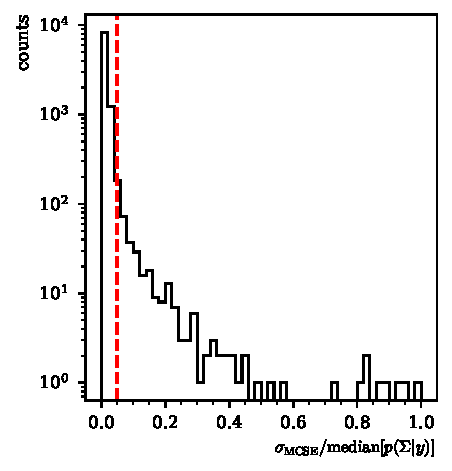
\includegraphics[width=.49\linewidth]{../bayes/toyMC/plots/toyMC_mcse_hist.pdf}
	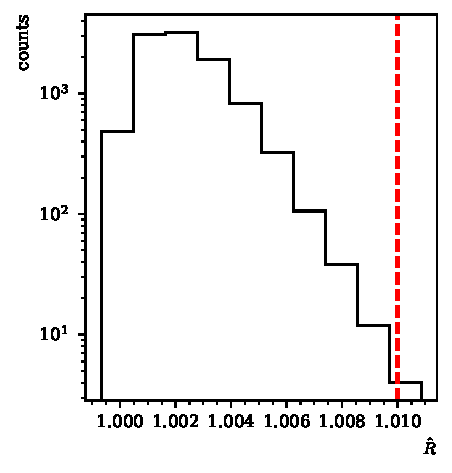
\includegraphics[width=.49\linewidth]{../bayes/toyMC/plots/toyMC_rhat_hist.pdf}
	\caption{ Left: relative error $\frac{\sigma_\text{MCSE}}{\text{median}\left[p\left(\Sigma|y\right)\right]}$ Right: $\widehat{R}$ associated with the fit parameter $\Sigma$. Both are shown for all 10000 fits. The critical values that should not be exceeded are marked by dashed lines.}
	\label{fig:toyMC_diagnostics}
\end{figure}
\subsubsection{Event based fit}
Not only signal events but also contributions from random time background as well as the imperfect detector efficiency $\epsilon(\phi)$ have to be simulated in order to test the method of event based fitting. For each polarization setting prompt peak and sideband events are drawn from the theoretical $\phi$-distributions $p_\text{prompt}$ and $p_\text{sideband}$ which are given in Equations \eqref{eq:pprmpt} and \eqref{eq:pside}. The total number of draws per setting and bin is again given by \textsc{Poisson} distributions and the ratio of prompt peak to sideband events is given by the time cut weights $\left\{w_i\right\}_{i=1}^7$ employed for the actual analysis of the $p\eta$ final state data \cite{farahphd}. This means that seven times prompt peak and sideband events need to simulated. The fraction of background events within the prompt peak $f$ was set to $f=0.95$. Further, the values $p_\gamma^\parallel=0.25,p_\gamma^\bot=0.3,\Sigma=0.5$, $\Sigma^\text{bkg}=-0.5$ and lastly, a random efficiency function as already chosen in reference \cite{farahphd} were appointed. Table \ref{tab:mcsum} shows a summary of all toy Monte Carlo properties.
\begin{table}[htbp]

	\renewcommand{\arraystretch}{1.5}
	\centering
	\begin{tabularx}{\linewidth}{l|XXX}
		\toprule
		\textbf{chosen parameters} & \multicolumn{3}{l}{$p_\gamma^\parallel=0.25,p_\gamma^\bot=0.3,\Sigma=0.5$, $\Sigma^\text{bkg}=-0.5$, $f=0.95$,}\\ &\multicolumn{3}{l}{$w_1=\frac{15}{210},w_2=\frac{8}{210},w_3=\frac{4}{210},w_4=\frac{10}{210},w_5=\frac{14}{210},w_6=\frac{6}{210},w_7=\frac{11}{210}$}\\
		\hline
		\textbf{simulation draws} &\multicolumn{3}{c}{$7\cdot N^\parallel_{\text{total},i}\sim\mathcal{P}(800)$, $7\cdot N^\bot_{\text{total},i}\sim\mathcal{P}(1000)\quad\big|_{i=1}^7$}\\
		\cline{2-4}
		&signal in prompt&background in prompt& sideband \\
		&$N^{\parallel/\bot}_\text{total}\cdot f$&$N^{\parallel/\bot}_\text{total}\cdot\left(1-f\right)$&$N^{\parallel/\bot}_\text{total}\cdot\left(1-f\right)\cdot1/w_i$\\
		\hline
		\textbf{efficiency function}&\multicolumn{3}{l}{$\epsilon\left(\phi\right)=1/10.5\cdot\left(9.3+0.28\cdot\cos\phi+0.24\cdot\sin3\phi\right)$}\\
		\bottomrule
	\end{tabularx}
	\caption{Summary of the complete setting of all toy Monte Carlo experiments for the event based fit. Values and table layout adapted from \cite{farahphd}.}
	\label{tab:mcsum}
\end{table}
In total, 1000 toy Monte Carlo experiments are thrown. To evaluate the fit results only the posterior distributions are available. As before, the residuals $\Xi$ are built from all fits, now for $\Sigma$ as well as $\Sigma^\text{bkg}$. They are shown in Figure \ref{fig:toyMC_diagnostics1} together with the unnormalized posterior distributions. Also the event based fit is able to reproduce the true values within one standard deviation. Only slight bias towards smaller values of the beam asymmetry is seen, but again with negligible effect on the results in comparison to the widths of the distributions. If the total amount of posterior distributions is not too large one might also combine them in a \emph{pooled likelihood} approach. $\dots$ This is shown in Figure \ref{fig:poollik} for both determined asymmetries. Because the true asymmetries are within $1\sigma$ of the resulting distribution one can finally conclude that the event based fit estimates positions and widths of the posterior distributions correctly.

\begin{figure}[htbp]
	\centering
	\begin{subfigure}{\linewidth}
		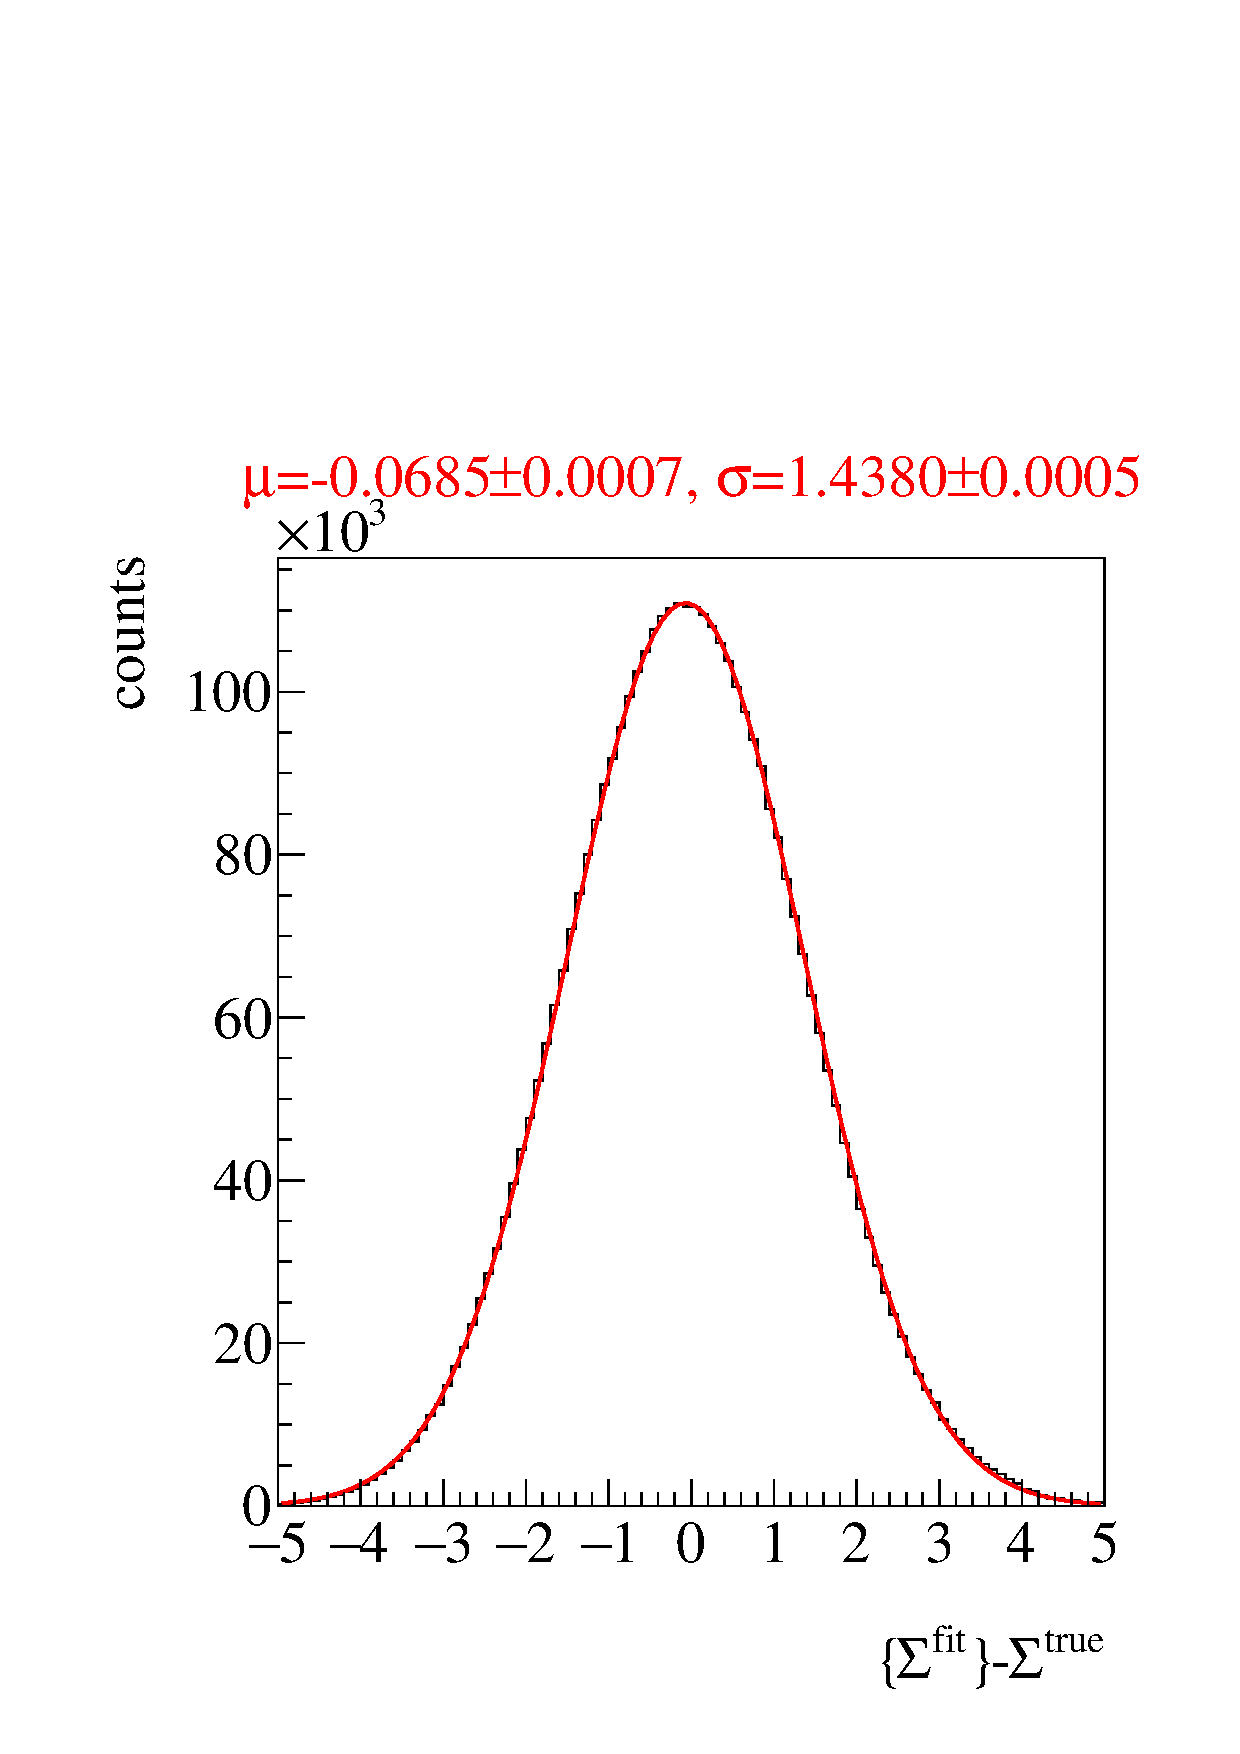
\includegraphics[width=.49\linewidth]{../bayes/event_based_fit/plots/combined_post_add.pdf}
		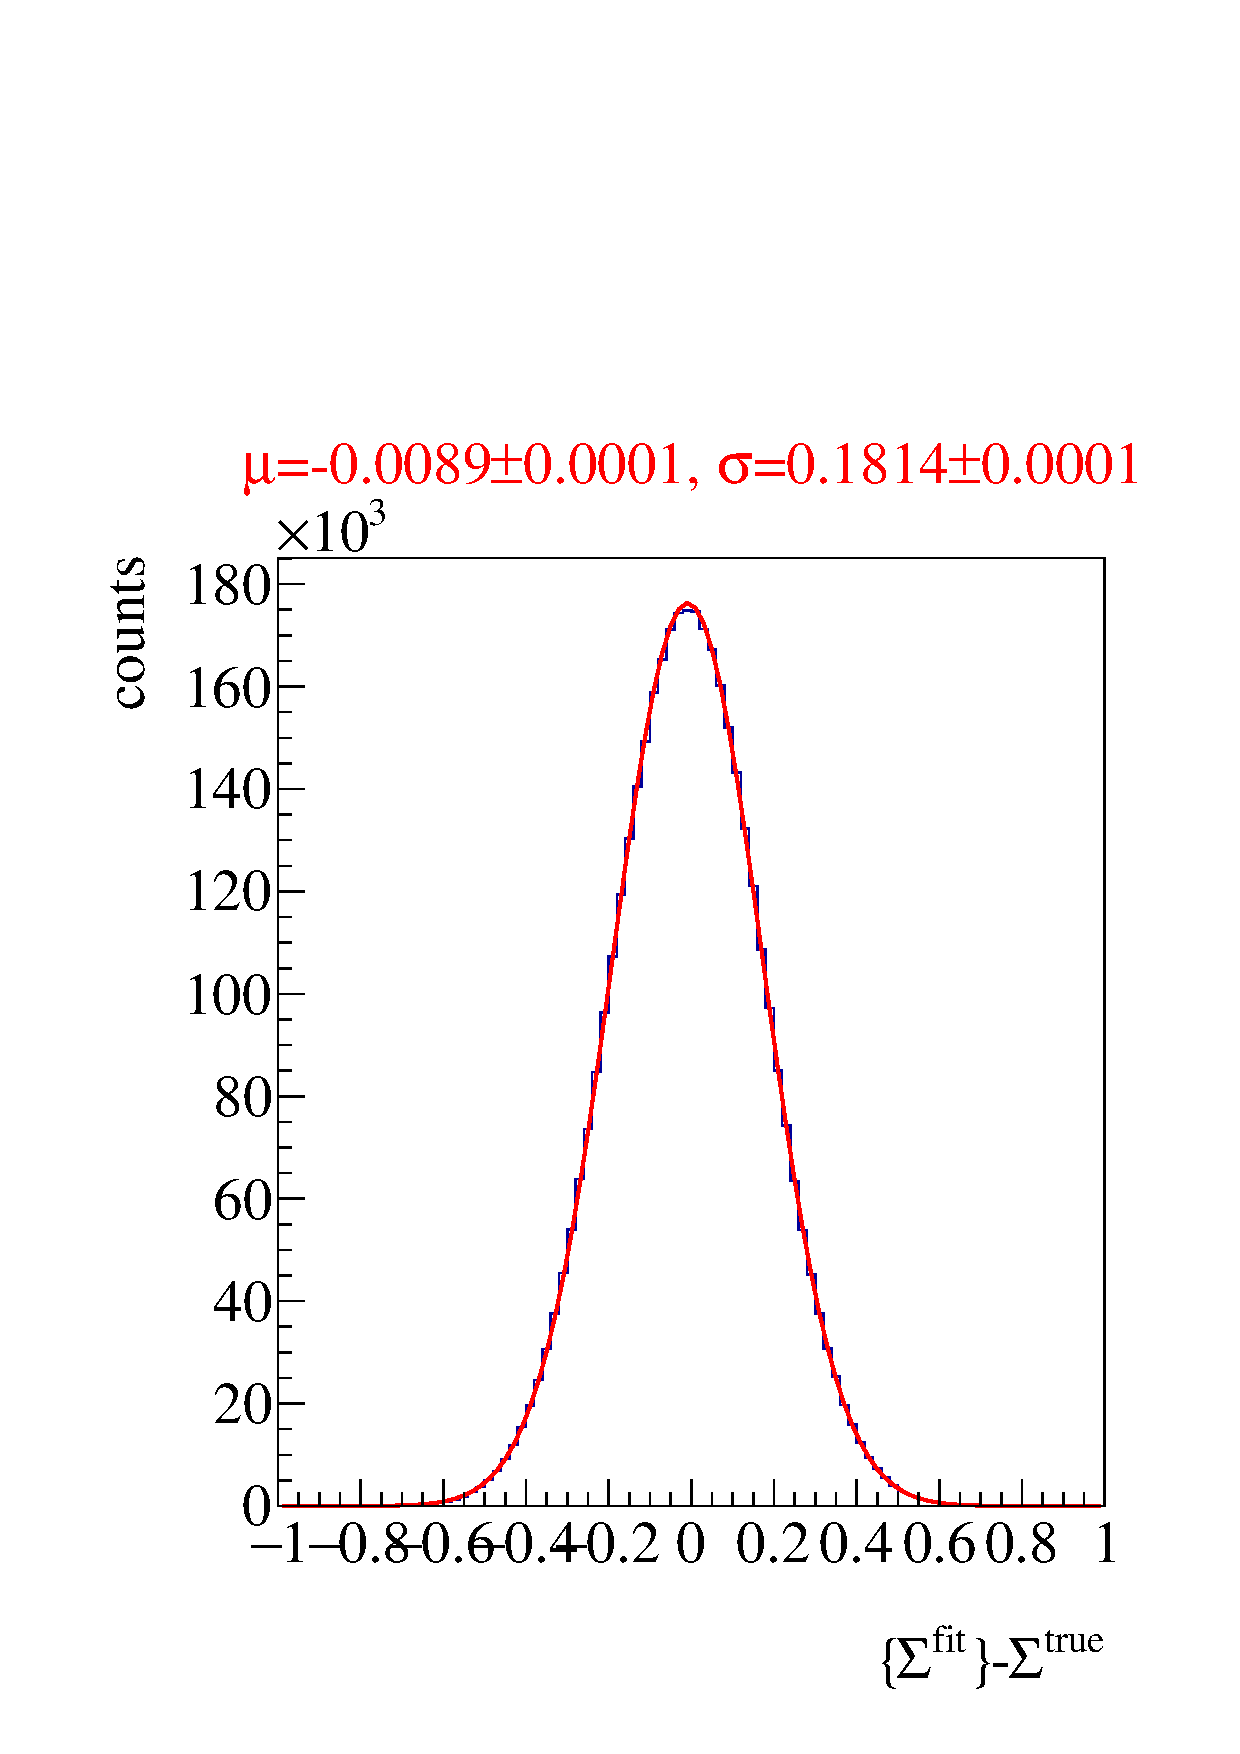
\includegraphics[width=.49\linewidth]{../bayes/event_based_fit/plots/combined_post_add_raw.pdf}
		\subcaption{Signal beam asymmetry $\Sigma$}
	\end{subfigure}
	\begin{subfigure}{\linewidth}
		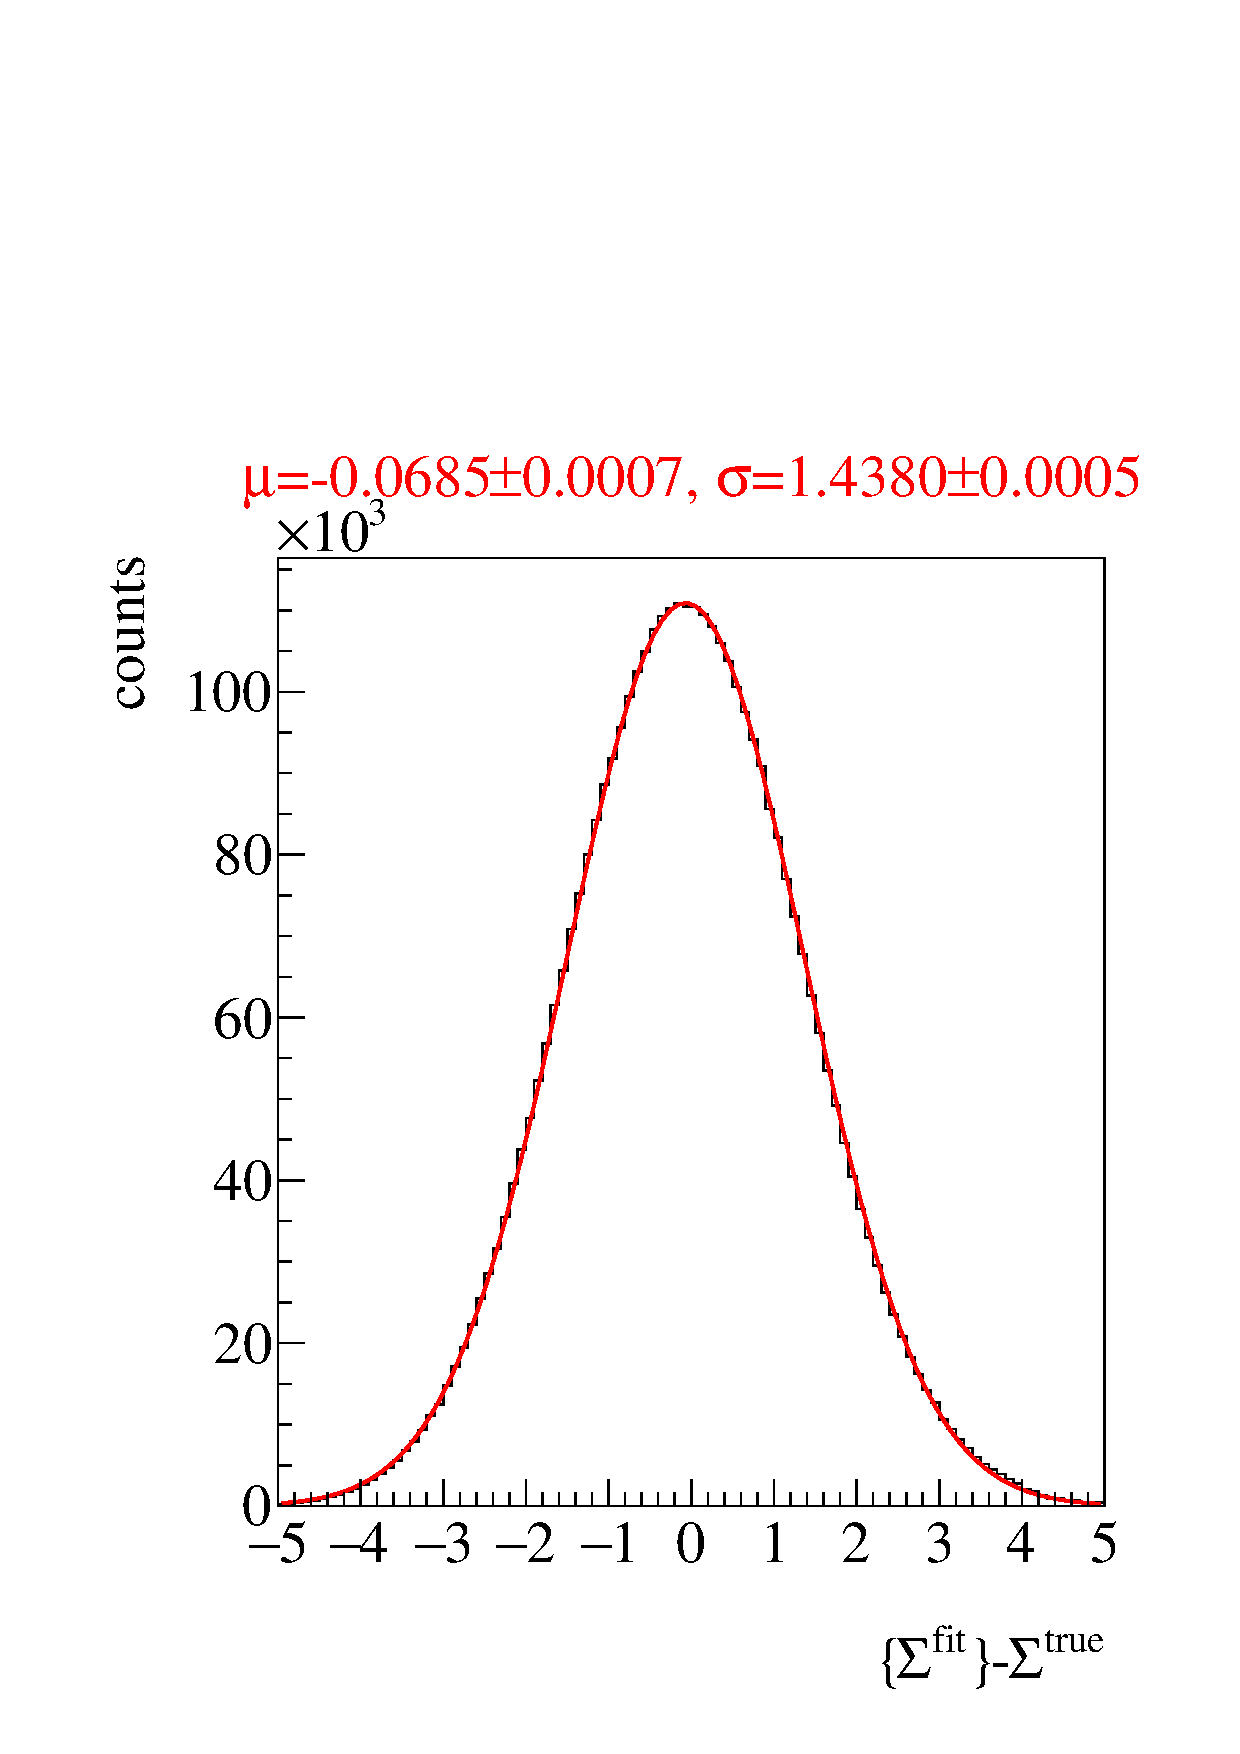
\includegraphics[width=.49\linewidth]{../bayes/event_based_fit/plots/combined_post_add.pdf}
		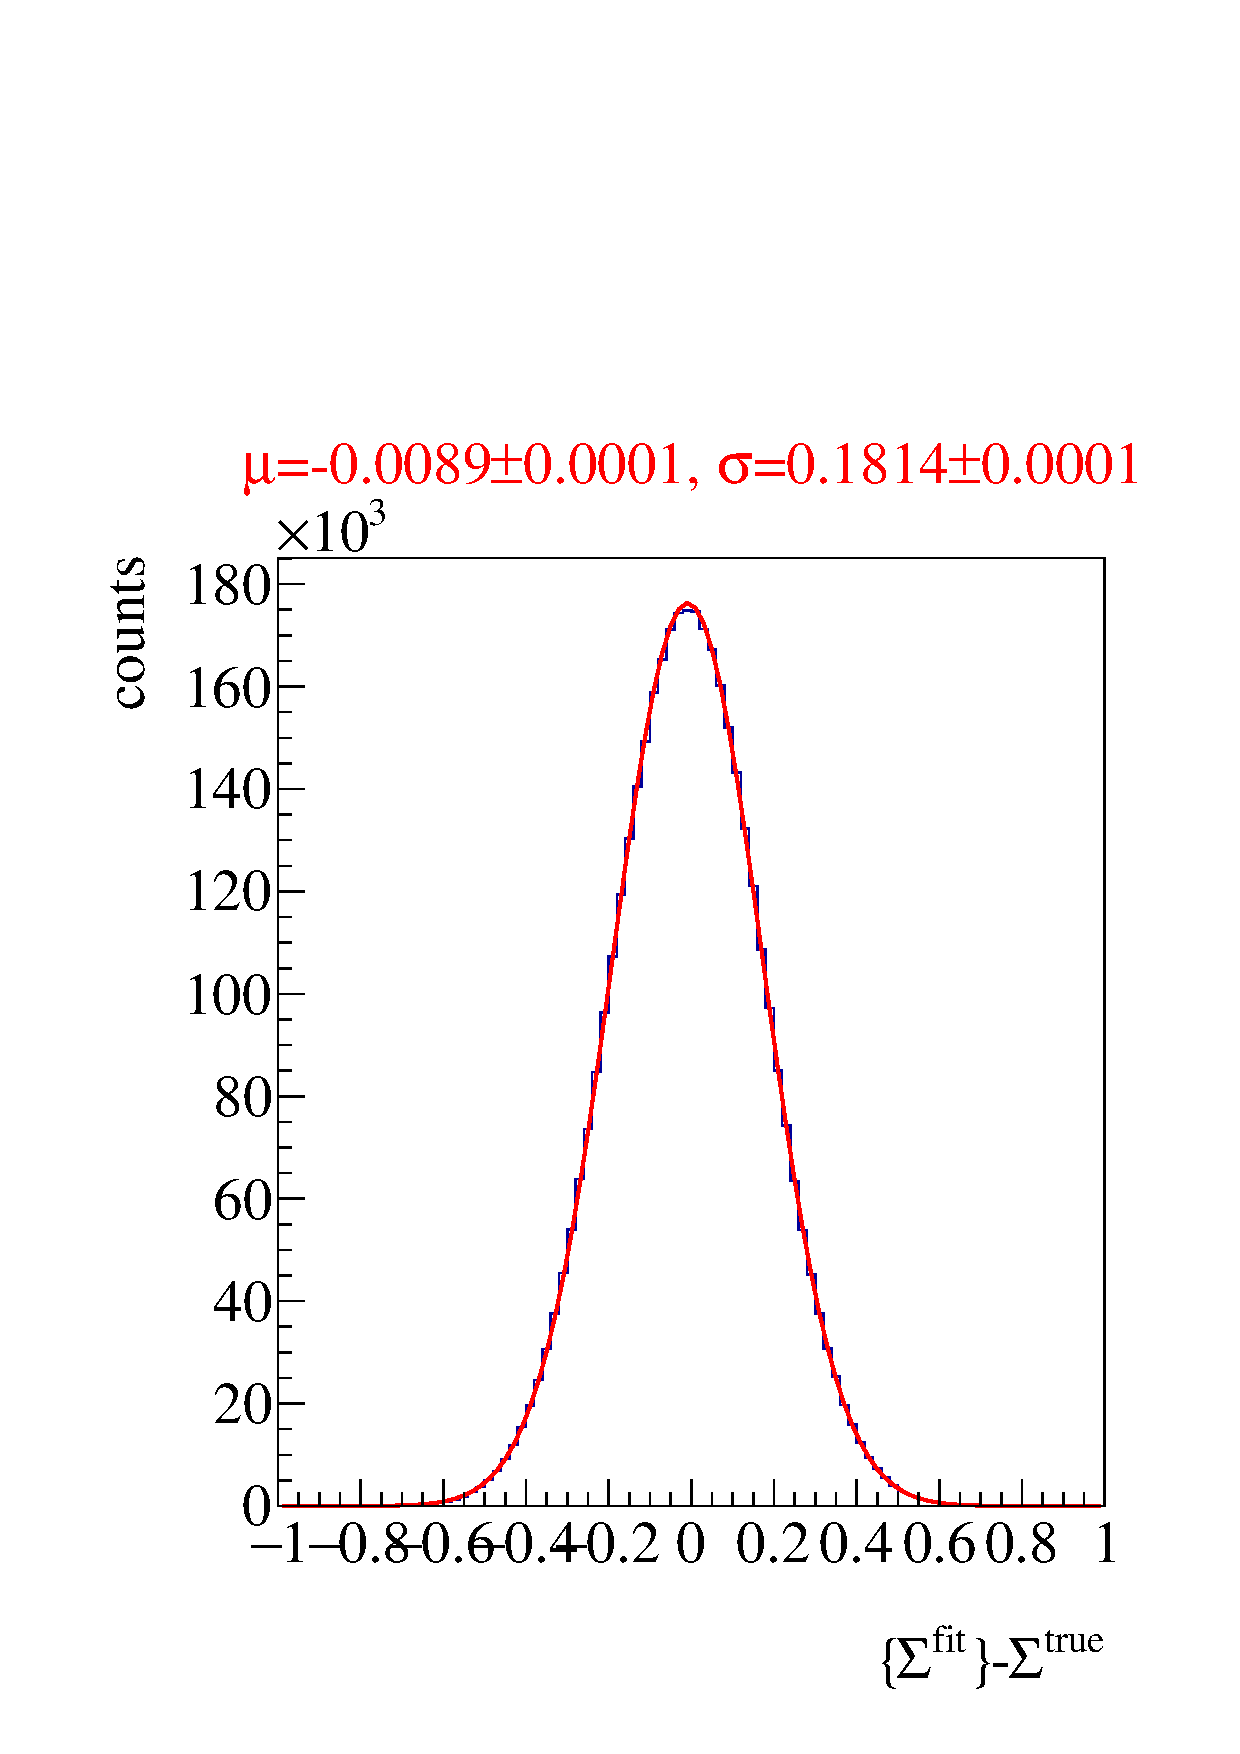
\includegraphics[width=.49\linewidth]{../bayes/event_based_fit/plots/combined_post_add_raw.pdf}
		\subcaption{Background beam asymmetry $\Sigma^\text{bkg}$}
	\end{subfigure}
	\caption{Combined posteriors for the beam asymmetries $\Sigma$ and $\Sigma^\text{bkg}$ from all 1000 event based fits. Left: Residuals $\Xi$ Right: Unnormalized posterior distributions. A \textsc{Gaussian} fit is performed on the distributions with results for mean $\mu$ and standard deviation $\sigma$ on top.}
	
\end{figure}


\begin{figure}[htbp]
	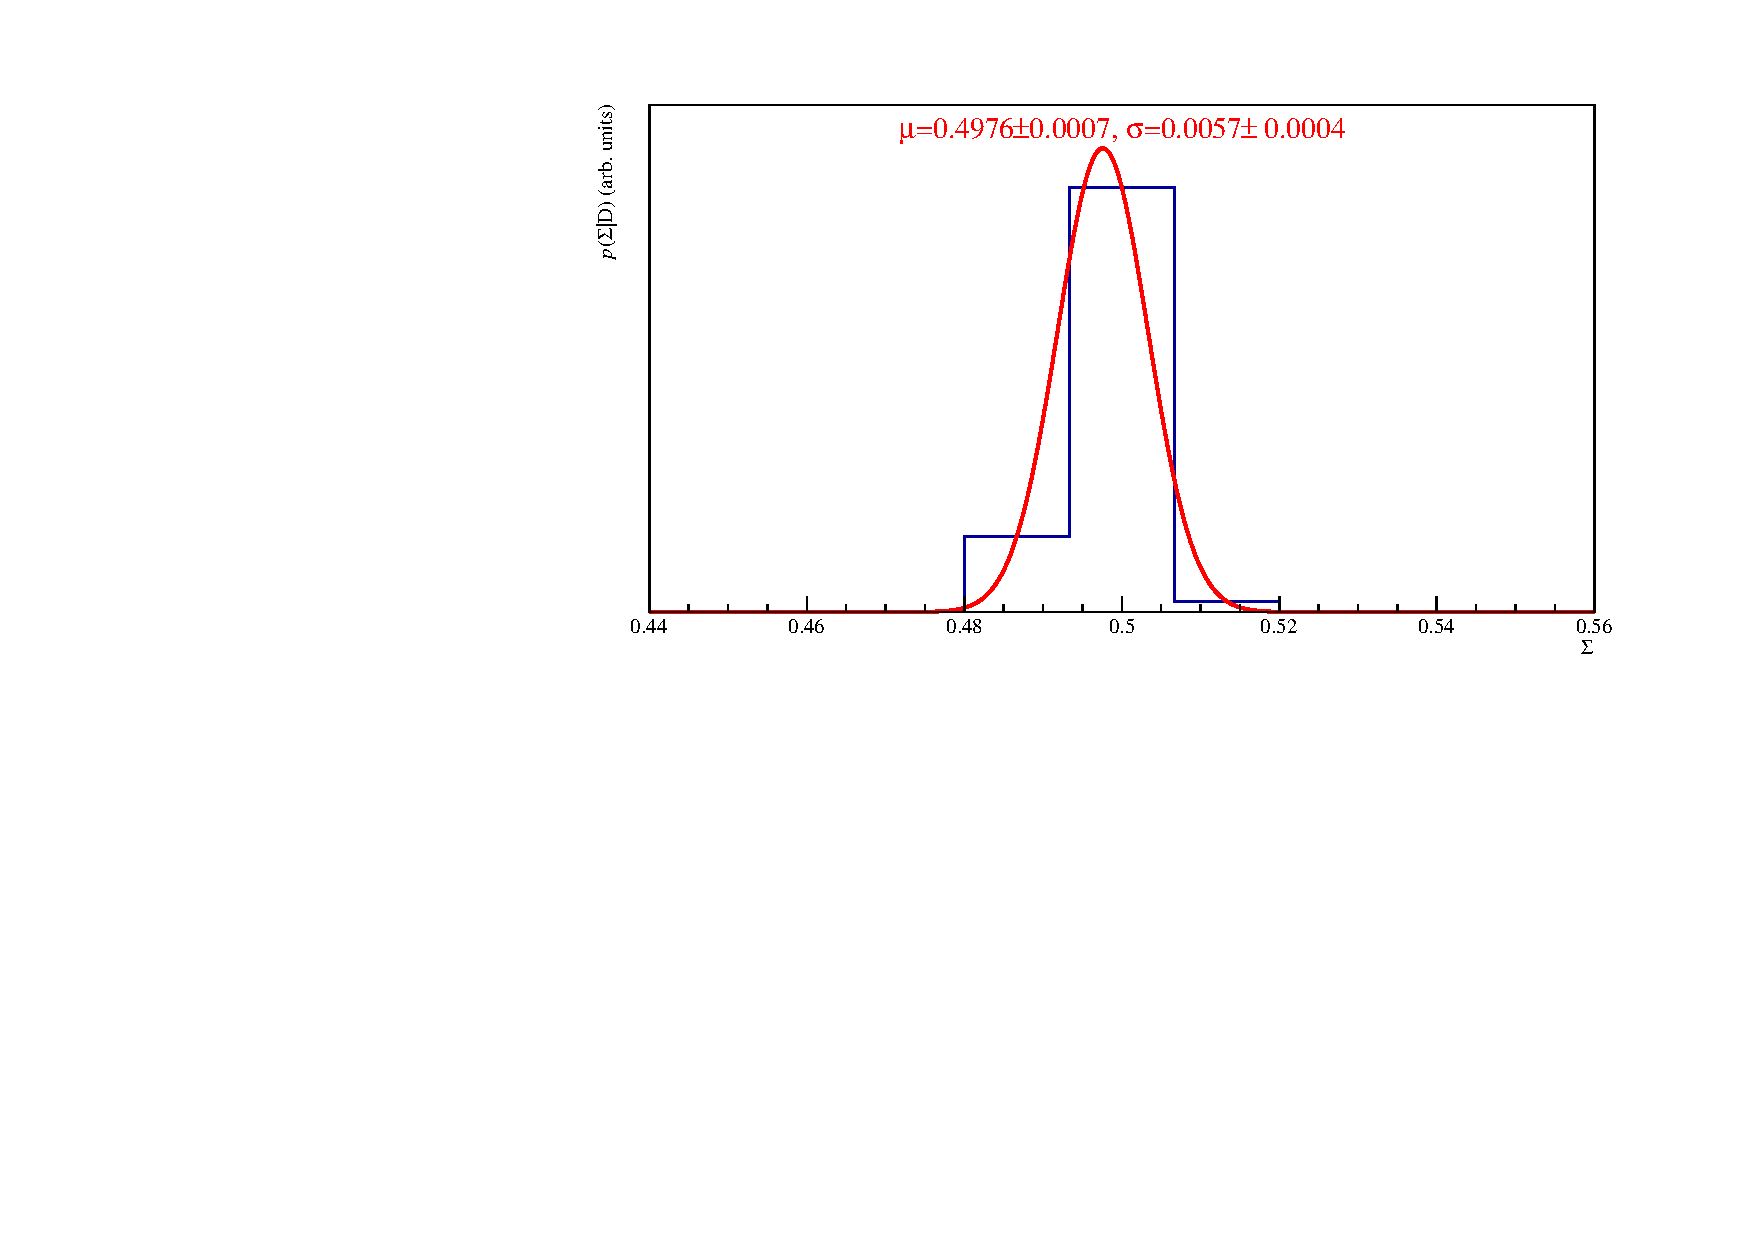
\includegraphics[width=.49\linewidth]{../bayes/event_based_fit/plots/combined_post_mul.pdf}
	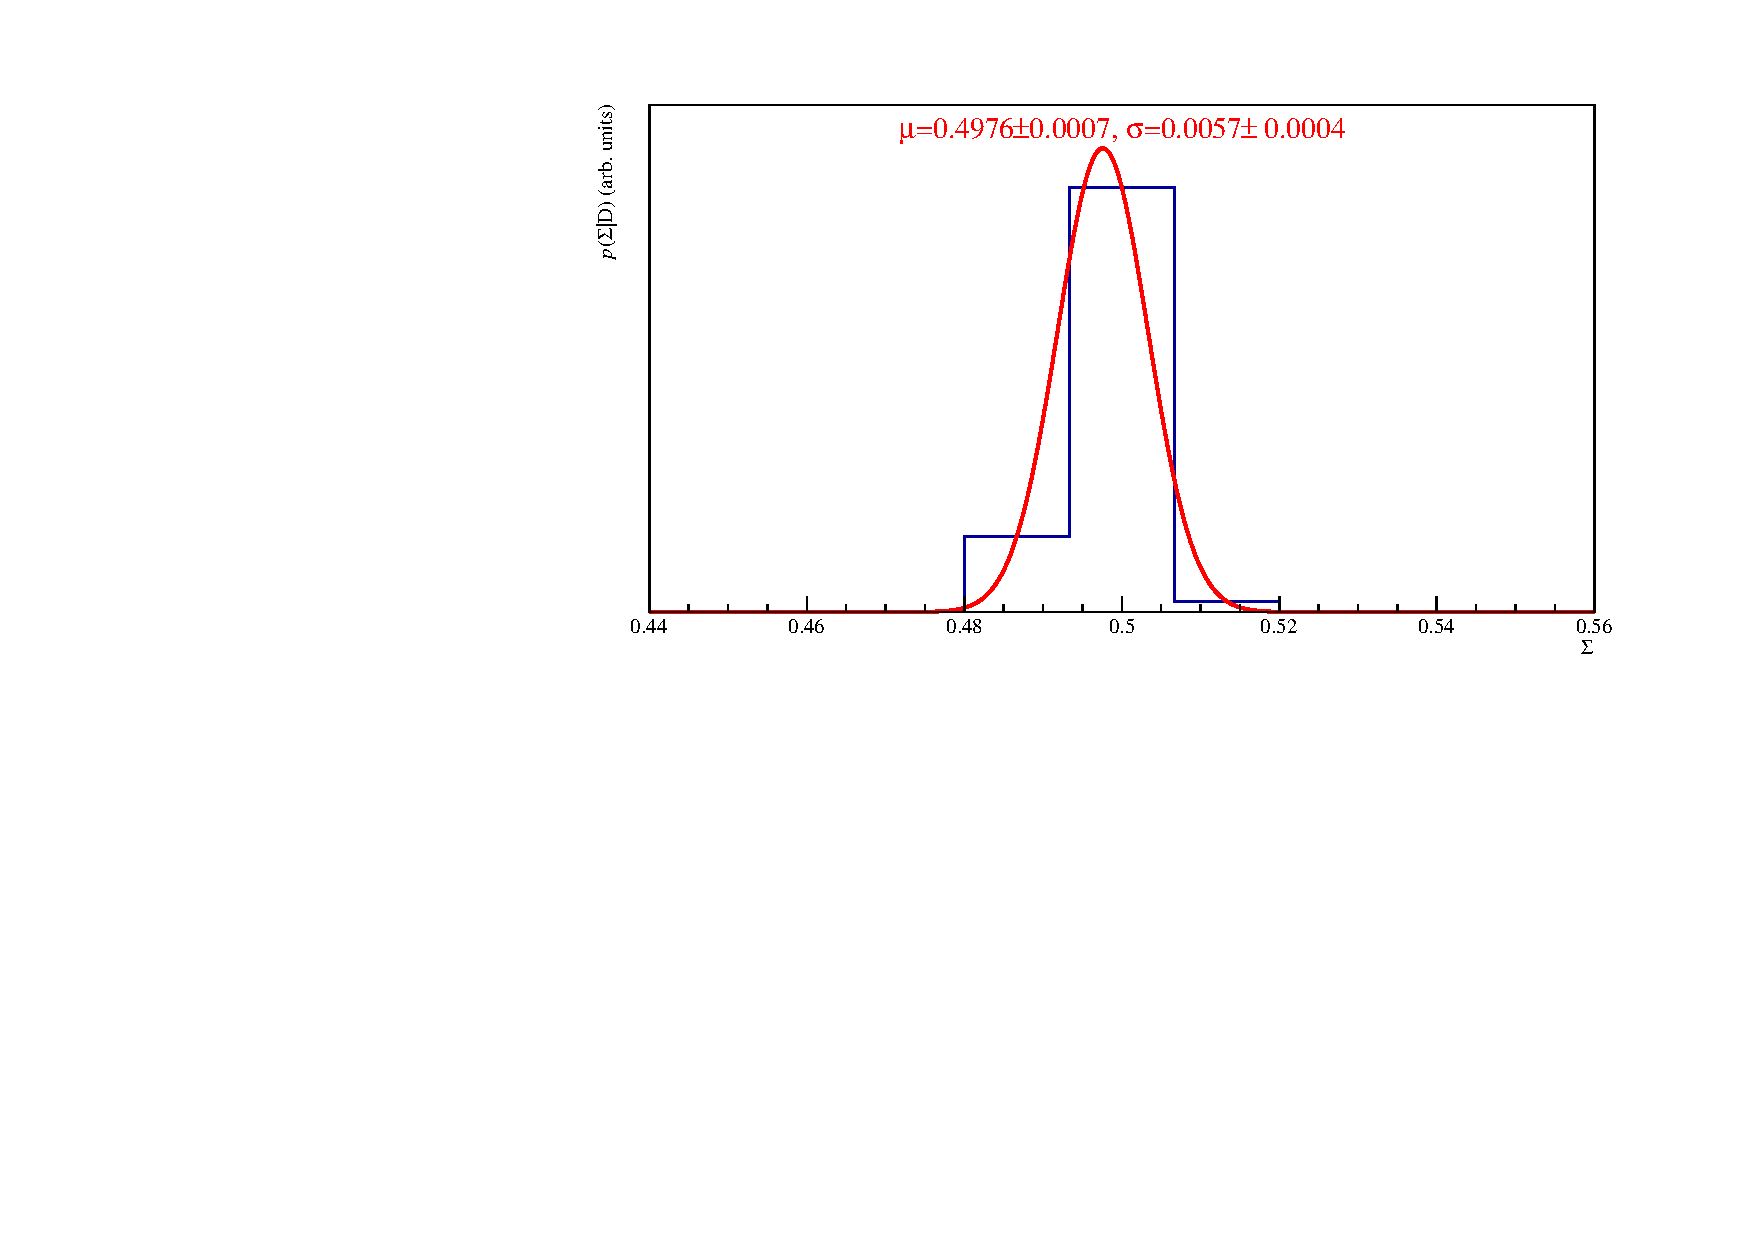
\includegraphics[width=.49\linewidth]{../bayes/event_based_fit/plots/combined_post_mul.pdf}
	\caption{Combined posterior probabilities using the \emph{pooled likelihood} approach. Left: Signal beam asymmetry, Right: background beam asymmetry. Mean and standard deviation as obtained from a \text{Gaussian} fit are shown on top}
	\label{fig:poollik}
\end{figure}
\begin{figure}[htbp]
	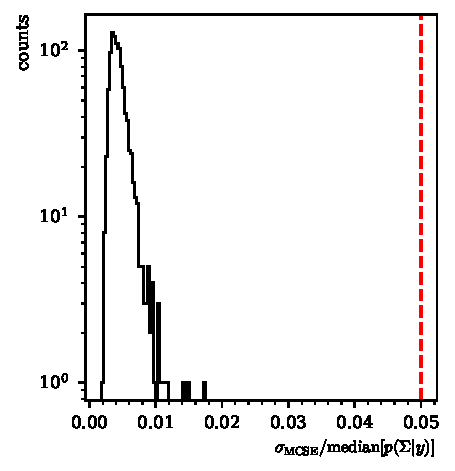
\includegraphics[width=.49\linewidth]{../bayes/event_based_fit/plots/toyMC_mcse_hist.pdf}
	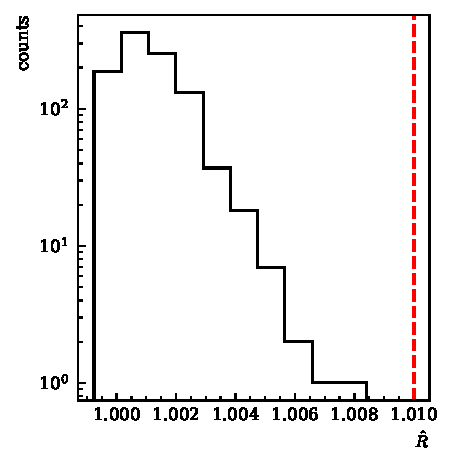
\includegraphics[width=.49\linewidth]{../bayes/event_based_fit/plots/toyMC_rhat_hist.pdf}
	\caption{ Left: relative error $\frac{\sigma_\text{MCSE}}{\text{median}\left[p\left(\Sigma|y\right)\right]}$ Right: $\widehat{R}$ associated with the fit parameter $\Sigma$. Both are shown for all 1000 fits. The critical values that should not be exceeded are marked by dashed lines.}
	\label{fig:toyMC_diagnostics1}
\end{figure}
\subsection{Application of methods to data}
\subsubsection{Event yield asymmetries}
\subsubsection{Event based fit}
\subsection{Discussion}
\section{Determination of $\Sigma_{\eta'}$}
placeholder
\subsection{Application of event based fit to toy Monte Carlo data}
placeholder
\subsection{Application of event based fit to data}
placeholder
\subsection{Systematic Error}
placeholder